\documentclass[table]{article}
\usepackage[rgb,dvipsnames]{xcolor}
\usepackage{tikz}
\usepackage{iclr2017_conference,times}
\usepackage{amsmath, amsthm}
\usepackage[subscriptcorrection,mtpcal,amsbb]{mtpro2}
\usepackage{hyperref}
\usepackage{url}
\usepackage{enumitem}
\setlist{leftmargin=15pt}
\usepackage{inconsolata}
\usepackage{textcomp}
\usepackage{lastpage}
\cfoot{\thepage\ of \pageref{LastPage}}
\usepackage{makecell}
\usepackage{physics}
\usetikzlibrary{arrows,positioning,automata}
\usetikzlibrary{shapes.geometric}
\usepackage{float}
\usepackage{subcaption}
\usepackage{array}
\newcolumntype{L}[1]{>{\raggedright\let\newline\\\arraybackslash\hspace{0pt}}m{#1}}
\newcolumntype{C}[1]{>{\centering\let\newline\\\arraybackslash\hspace{0pt}}m{#1}}
\newcolumntype{R}[1]{>{\raggedleft\let\newline\\\arraybackslash\hspace{0pt}}m{#1}}
\usepackage{colortbl}
\usepackage{hhline}
\usepackage[labelfont=bf,labelsep=period]{caption}

\newcommand{\thickhline}{%
    \noalign {\ifnum 0=`}\fi \hrule height 1pt
    \futurelet \reserved@a \@xhline
}

\lhead{\textsc{IFT6135 Representation Learning}}
\rhead{S. Laferri\`ere \& J. Litalien}

\title{Assignment 4 --- Practical Part \\
Generative Models (GANs)}
\author{Samuel Laferri\`ere\thanks{Student ID P0988904}\ \, \& Joey Litalien\thanks{Student ID P1195712} \\
IFT6135 Representation Learning, Winter 2018\\
Universit\'e de Montr\'eal\\
Prof. Aaron Courville \\
\texttt{$\{$samuel.laferriere.cyr,joey.litalien$\}$@umontreal.ca}}

\def\*#1{\mathbf{#1}}
\DeclareMathOperator{\ex}{\mathbb{E}}
\DeclareMathOperator{\Var}{Var}

\newcommand{\code}[1]{{\color{Blue}\small\texttt{#1}}}

\begin{document}
\maketitle
\thispagestyle{empty}

\section{Overview}

For this assignment, we chose to implement a Generative Adversarial Network (GAN) in PyTorch. The variant we used for comparison is a Wasserstein GAN (WGAN). The class \code{DCGAN} implements a Deep Convolutional GAN and contains both a \code{Discriminator} $D$ and \code{Generator} $G$. Both entities can be trained independently using the methods \code{DCGAN.train\_*}, meaning that we can customize the order in which we train the models. These training routines implement two types of loss functions: the original minmax loss from Goodfellow (2014), and the Wasserstein version from Arjovsky (2017). Every hyperparameters related to training like $D$'s and $G$'s optimizers are set in \code{CelebA}, a wrapper class for the generative task at hand.

To load a pre-trained model, simply instantiate \code{CelebA} with the default parameters, load the model weights and call \code{DCGAN.generate\_img()}. If no arguments is passed, the GAN will sample a random latent variable $\*z$ and return a generated image. This function also accepts a latent variable generated from a fixed RNG seed.

\section{Architecture}
\subsection{DCGAN}

We reused the DCGAN architecture from Radford (2015) to build our vanilla GAN. The architectures for the discriminator and generator are given in the tables below. The last three columns are kernel size, stride and padding, respectively.

\begin{table}[ht]
\centering
\begin{tabular}{c c ccc c c c}
\Xhline{2\arrayrulewidth}
In & Out & Module & Normalization & Activation & $k$ & $s$ & $p$ \\
\hline
100 & 1024 &Deconv2D & BatchNorm2D & ReLU & $4 \times 4$ & 1 & 0 \\
1024 & 512 &Deconv2D & BatchNorm2D & ReLU & $4 \times 4$ & 2 & 1 \\
12 & 256 &Deconv2D & BatchNorm2D & ReLU & $4 \times 4$ & 2 & 1 \\
128 & 128 &Deconv2D & BatchNorm2D & ReLU & $4 \times 4$ & 2 & 1 \\
28 & 3 &Deconv2D & --- & Tanh & $4 \times 4$ & 2 & 1 \\
\Xhline{2\arrayrulewidth}
\end{tabular}
\caption{DCGAN Generator architecture.}
\end{table}

\begin{table}[ht]
\centering
\begin{tabular}{c c ccc c c c}
\Xhline{2\arrayrulewidth}
In & Out & Module & Normalization & Activation & $k$ & $s$ & $p$ \\
\hline
3 & 128 &Conv2D & --- & LeakyReLU(0.2) & $4 \times 4$ & 2 & 1 \\
128 & 256 &Conv2D & BatchNorm2D & LeakyReLU(0.2) & $4 \times 4$ & 2 & 1 \\
256 & 512 &Conv2D & BatchNorm2D & LeakyReLU(0.2) & $4 \times 4$ & 2 & 1 \\
512 & 1024 &Conv2D & BatchNorm2D & LeakyReLU(0.2) & $4 \times 4$ & 2 & 1 \\
1024 & 1 & Conv2D & BatchNorm2D & Sigmoid & $4 \times 4$ & 1 & 0 \\
\Xhline{2\arrayrulewidth}
\end{tabular}
\caption{DCGAN Discriminator architecture.}
\end{table}

As suggested in the paper, we did not apply batchnorm to $G$'s output layer and $D$'s input layer to avoid sample oscillation and model instability.

We further detail our choice of hyperparameters as follows.


\begin{table}[ht]
\centering
\begin{tabular}{l C{1.5cm} c}
\Xhline{2\arrayrulewidth}
Hyperparameter & Symbol & Value \\
\hline
Learning rate & $\alpha$ & 0.0002 \\
Momentum & $\beta, \beta^2$ & 0.5, 0.999\\
SGD Optimizers & --- & Adam \\
$D/G$ updates ratio & $n_{\textsf{critic}}$ & 3:1 \\
\hline
Image size & $d$ & $3 \times 64 \times 64$ \\
Training size & $N$ & 202,599\\
Batch size & $b$ & 128 \\
\Xhline{2\arrayrulewidth}
\end{tabular}
\caption{DCGAN Choice of hyperparameters.}
\end{table}

\subsection{Increasing the Feature Map Size}

\newpage
\section{Qualitative Evaluations}
\subsection{DCGAN vs. WGAN Visual Comparison}


\subsection{Latent Space Exploration}
To explore the face manifold in latent space, we iterated over all $10^2$ dimensions of two given $\*z$'s and changed the value to $\pm 3\sigma^2 = \pm 3$ to amplify the signal. We selected the dimensions we thought gave the most notable differences. Among the visual variations we observed are open/close mouth, skin color, hair fringe, hair colour, cheek and jaw shape, background, and gender changes. Interestingly, we also have a semblance of face orientation change in the woman case (first and fourth from the right).
\begin{figure}[ht]
  \centering
  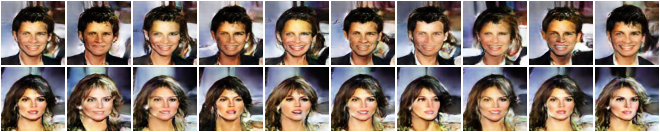
\includegraphics[width=\textwidth]{imgs/latent_explore}
  \caption{DCGAN: Changing a single dimension in latent space. Original face $\*x = G(\*z)$ is the left-most image.}
\end{figure}

\subsection{Screen and Latent Space Interpolation}
Interpolating in screen space (Figure \ref{screen_lerp}) obviously gave very poor results as we simply interpolate between pixels and completely disregard the underlying structure of the generator $G$. Only the first and last images look like actual human faces; anything in the middle has ghosting artifacts since it is just a blend of RGB channels.

\begin{figure}[ht]
  \centering
  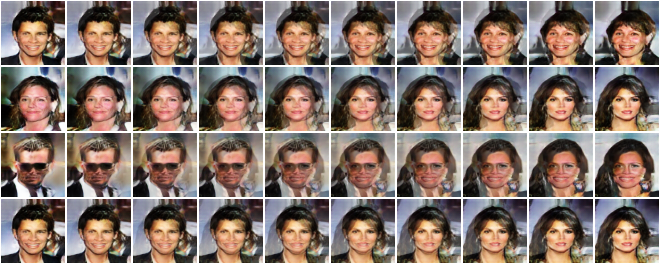
\includegraphics[width=\textwidth]{imgs/gan_screen_lerp}
  \caption{DCGAN: Interpolating in screen space: $\*x' = \alpha \*x_0 + (1-\alpha)\*x_1, \ \alpha \in [0,1]$.}
  \label{screen_lerp}
\end{figure}

Interpolating in latent space (Figure \ref{latent_lerp}), however, gives pleasant results. Indeed, any $\*z'$ seems to yield a plausible celebrity face. This is because when we interpolate the latent variables, we ``walk" on the face manifold of $G$ and so any value should somewhat give a realistic face.

To better visualize the interpolation process, we created looping GIFs (and MP4 videos to avoid compression artifacts) over 50 frames (\textit{i.e.} $\alpha = i/50$). These are located in the \code{explore/screen\_space} and \code{explore/latent\_space} directories of the project source.


\begin{figure}[ht]
  \centering
  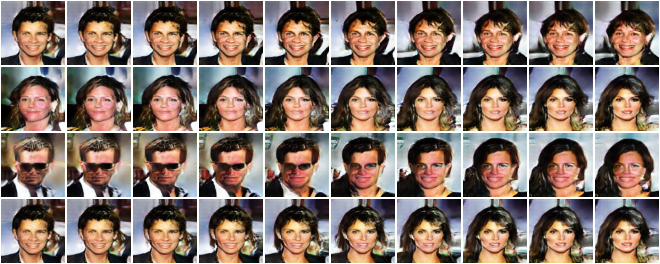
\includegraphics[width=\textwidth]{imgs/gan_latent_lerp}
  \caption{DCGAN: Interpolating in latent space: $\*z' = \alpha \*z_0 + (1-\alpha)\*z_1, \ \alpha \in [0,1]$.}
  \label{latent_lerp}
\end{figure}

\section{Quantitative Evaluations}




\end{document}
